
% This LaTeX was auto-generated from an M-file by MATLAB.
% To make changes, update the M-file and republish this document.

\documentclass{article}
\usepackage{graphicx}
\usepackage{color}
\usepackage{listings}
\usepackage[framed]{mcode}
\usepackage{fullpage}
\usepackage{hyperref}
\usepackage{amsmath}

\definecolor{lightgray}{gray}{0.5}
\setlength{\parindent}{0pt}

\begin{document}
    
%\section*{}

\begin{par}

\title{BE 521 - Homework 7\\{\normalsize Spring 2015}}
\author{Mike Lautman}
\date{\today}
\maketitle
\textbf{Objective:} Motor Prediction

\end{par}
\begin{par}

\section*{0 Setup}

\end{par}
\begin{lstlisting}
clf; close all; clear; clc;
addpath(genpath('./libsvm-3.20/matlab/'));
me = 'mlautman';
pass_file = 'mla_ieeglogin.bin';

dataset1 = 'I521_A0007_D001';
dataset2 = 'I521_A0007_D002';
[T, session1] = evalc('IEEGSession(dataset1, me, pass_file)');
[T, session2] = evalc('IEEGSession(dataset2, me, pass_file)');
data1 = session1.data;
data2 = session2.data;
sr1 = data1.sampleRate;     % Hz
Nvals1 = data1.channels(1).get_tsdetails.getNumberOfSamples;
Nvals2 = data2.channels(1).get_tsdetails.getNumberOfSamples;
neurons = data1.getvalues(1:Nvals1, 1:40);
positions = data2.getvalues(1:Nvals2, 1:2);
\end{lstlisting}
\begin{par}

\section*{1 Motor Predictions}

\end{par}
\begin{par}

\subsection*{1.1 R size}
The correct size of $R$ is $1972 x  801$ since there are $1972$ x-y
position values and $40 neurons * 20 time bins + 1 for bias$

\end{par}
\begin{lstlisting}
N = 20; % backwards looking time stamps for each neuron for feature vect
d = 40 * N + 1; % 40 neurons by 20 time steps plus a ones vect for bias
M = 1972; % last timestamp for positions

R = zeros(M, d);
size(R)
\end{lstlisting}

\color{lightgray} \begin{lstlisting}
ans =

        1972         801

\end{lstlisting} \color{black}
\begin{par}

\subsection*{1.2 Generate the R matrix}

\end{par}
\begin{lstlisting}
% We create the R matrix
for i=1:M
    e = i + N - 1;
    row = neurons(i:e, :);
    R(i, :) = [1, row(:)'];
end

mean(mean(R))
\end{lstlisting}

\color{lightgray} \begin{lstlisting}
ans =

    1.5096

\end{lstlisting} \color{black}
\begin{par}

\subsection*{1.3 linear filter}

\end{par}
\begin{lstlisting}
% Training data
s = positions;

% Linear regression explicit solution
f = (R' * R) \ (R' * s);
\end{lstlisting}
\begin{par}

\subsection*{1.3.a Show Weights}

\end{par}
\begin{lstlisting}
% plotting
f_len = length(f);
f_x = f(2:f_len,1);
f_x2 = reshape(f_x, [20,40])';
figure(1)
imagesc(f_x2)
colorbar()
title('Weight matrix for X position')
xlabel('Time bin')
ylabel('Neuron #')

f_y = f(2:f_len,2);
f_y2 = reshape(f_y, [20,40])';
figure(2)
imagesc(f_y2)
colorbar()
title('Weight matrix for Y position')
xlabel('Time bin')
ylabel('Neuron #')
\end{lstlisting}


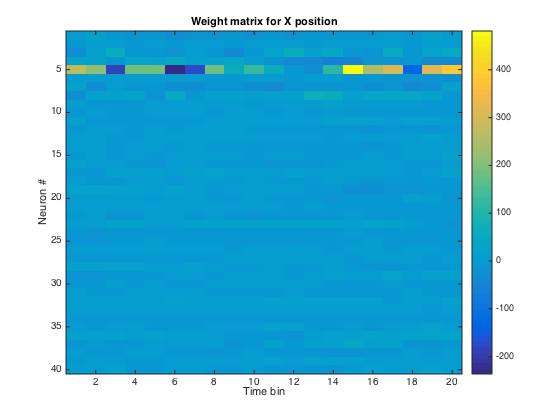
\includegraphics [width=4in]{mlautman_hw7_01.png}


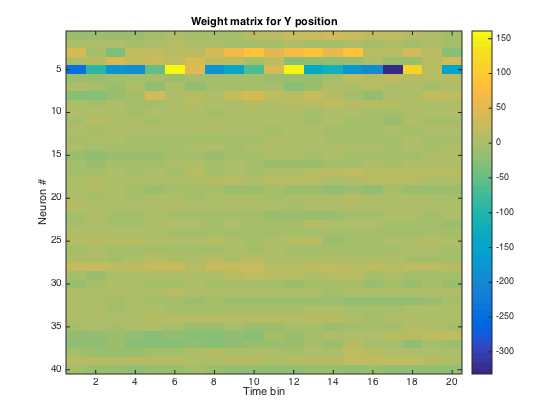
\includegraphics [width=4in]{mlautman_hw7_02.png}
\begin{par}

\subsection*{1.3.b Notes on the Weight Vector}
We can clearly see that our linear regression is very heavily dependent
on neuron 5 to predict the correct position of the hand. We can also see
that the variance in weight is very evenly spread out among the rest of
the neurons. This leads us to believe that either neuron 5 by far the
most important neuron for predicting the position of the monkey's hand or
our linear regression model is overfitting. Overfitting might occur if
the true decision function is too complex for us to get a good
generalizable prediction function from a simple model such as linear
regression.

\end{par}
\begin{par}

\subsection*{1.4 Predictions}

\end{par}
\begin{lstlisting}
% predictions
u = R * f;
\end{lstlisting}
\begin{par}

\subsection*{1.4.a Plot Predictions}

\end{par}
\begin{lstlisting}
% plotting
figure(3)
subplot(2,1,1)
hold on
plot((1:length(s(:,1))) * .070, s(:,1), 'b')
plot((1:length(u(:,1))) * .070, u(:,1), 'r')
title('X Position')
legend('True X position', 'Predicted X position', 'Location', 'best')
xlabel('Time (S)')
ylabel('X Position (Unknown units)')

subplot(2,1,2)
hold on
plot((1:length(s(:,2))) * .070, s(:,2), 'b')
plot((1:length(u(:,2))) * .070, u(:,2), 'r')
title('Y Position')
legend('True Y position', 'Predicted Y position', 'Location', 'best')
xlabel('Time (S)')
ylabel('Y Position (Unknown units)')
\end{lstlisting}


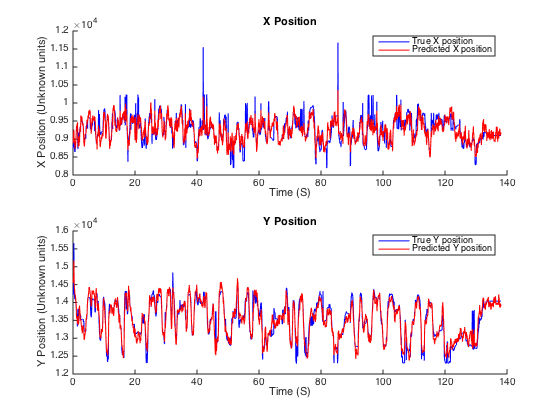
\includegraphics [width=4in]{mlautman_hw7_03.png}
\begin{par}

\subsection*{1.4.b $\rho x$ and $\rho_{y}$}

\end{par}
\begin{lstlisting}
rho_x = corr(s(:,1),u(:,1))
rho_y = corr(s(:,2),u(:,2))
\end{lstlisting}

\color{lightgray} \begin{lstlisting}
rho_x =
    0.8389


rho_y =
    0.9556

\end{lstlisting} \color{black}
\begin{par}

\subsection*{1.5 Animating Motion (commented out for convenience)}

\end{par}
\begin{lstlisting}
 figure(4)
 for i=1:length(s)
 	scatter(s(i,1), s(i,2), 'ro')
 	hold on
 	scatter(u(i,1), u(i,2), 'b.')
 	hold off
 	xlim([8000 12000])
 	ylim([12000 16000])
 	pause(.035)
 end
\end{lstlisting}
\begin{par}

\section*{2 A More Realistic Setting}

\end{par}
\begin{par}

\subsection*{2.1 Test Set Accuracy}

\end{par}
\begin{lstlisting}
N = 20; % backwards looking time stamps for each neuron for feature vect
d = 40 * N + 1; % 40 neurons by 20 time steps plus a ones vect for bias
M = 1972; % last timestamp for positions
tst_len = 400;

% We create the R matrix
R = zeros(M, d);
for i=1:M
    e = i + N - 1;
    row = neurons(i:e, :);
    R(i, :) = [1, row(:)'];
end

% Turn on or off randomization
perm = randperm(size(R,1));
% perm = 1:size(R,1);

Rshuff = R(perm, :);
R_tst = Rshuff(1:tst_len,:);
R_trn = Rshuff(tst_len+1:size(Rshuff,1),:);

% Training data
s = positions(perm, :);
s_tst = s(1:tst_len,:);
s_trn = s(tst_len+1:length(s),:);

% Linear regression explicit solution
f_trn = pinv(R_trn' * R_trn) * (R_trn' * s_trn);

% predictions
u_trn = R_trn * f_trn;
u_tst = R_tst * f_trn;

% Solving for the correlation scores
rho2_x = corr(s_tst(:,1),u_tst(:,1))
rho2_y = corr(s_tst(:,2),u_tst(:,2))
\end{lstlisting}

\color{lightgray} \begin{lstlisting}
rho2_x =

    0.5149


rho2_y =

    0.8396

\end{lstlisting} \color{black}
\begin{par}

We see a large drop in the $\rho_{x}$ score while the $\rho_{y}$ score
only drops a little. This is expected since validating your model on the
testing set will inevitably give a higher accuracy than validating
against an unseen testing set. However, there are still issues with this
method. Since we did not randomize the rows for the training and test
sets, we could run into issues if moving average position of the hand
changes with time. (ie his hand was up for the first half and down for
the second) We would see an effect from such a bias in the histograms for
position in the testing and training sets. (shown below) Furthermore, by
plotting the predicted and true positions for the test data, we can see a
clear overfitting problem caused by the high variance of our predictions.

\end{par}
\begin{lstlisting}
figure(5)
hold on
histogram(s_trn(:,1), 'FaceColor', 'b')
histogram(s_tst(:,1), 'FaceColor', 'r')
title('X Positions Histogram in Testing and Training sets')
xlabel('X Position')
ylabel('Count')
legend('Training','Testing','Location', 'best')

figure(6)
hold on
histogram(s_trn(:,2), 'FaceColor', 'b')
histogram(s_tst(:,2), 'FaceColor', 'r')
title('Y Positions Histogram in Testing and Training sets')
xlabel('Y Position')
ylabel('Count')
legend('Training','Testing','Location', 'best')


% plotting
figure(7)
subplot(2,1,1)
hold on
plot((1:length(s_trn(:,1))) * .070, s_trn(:,1), 'b')
plot((1:length(u_trn(:,1))) * .070, u_trn(:,1), 'r')
title('Training X Position')
legend('True X position', 'Predicted X position', 'Location', 'best')
xlabel('Time (S)')
ylabel('X Position (Unknown units)')

subplot(2,1,2)
hold on
plot((1:length(s_trn(:,2))) * .070, s_trn(:,2), 'b')
plot((1:length(u_trn(:,2))) * .070, u_trn(:,2), 'r')
title('Training Y Position')
legend('True Y position', 'Predicted Y position', 'Location', 'best')
xlabel('Time (S)')
ylabel('Y Position (Unknown units)')

figure(8)
subplot(2,1,1)
hold on
plot((1:length(s_tst(:,1))) * .070, s_tst(:,1), 'b')
plot((1:length(u_tst(:,1))) * .070, u_tst(:,1), 'r')
title('Test X Position')
legend('True X position', 'Predicted X position', 'Location', 'best')
xlabel('Time (S)')
ylabel('X Position (Unknown units)')

subplot(2,1,2)
hold on
plot((1:length(s_tst(:,2))) * .070, s_tst(:,2), 'b')
plot((1:length(u_tst(:,2))) * .070, u_tst(:,2), 'r')
title('Test Y Position')
legend('True Y position', 'Predicted Y position', 'Location', 'best')
xlabel('Time (S)')
ylabel('Y Position (Unknown units)')
\end{lstlisting}


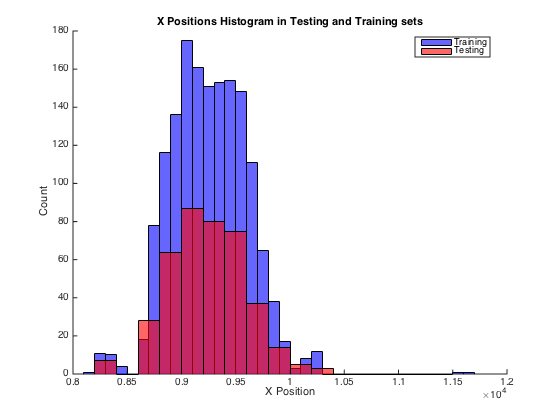
\includegraphics [width=4in]{mlautman_hw7_04.png}


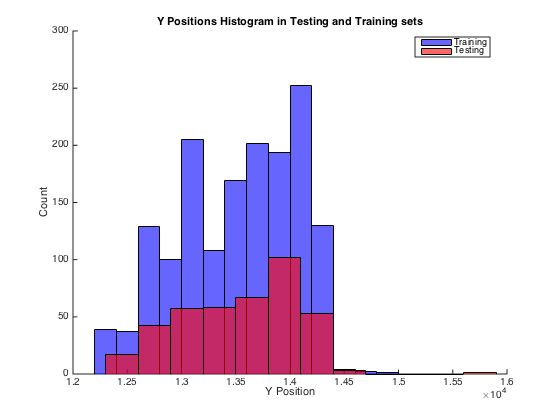
\includegraphics [width=4in]{mlautman_hw7_05.png}


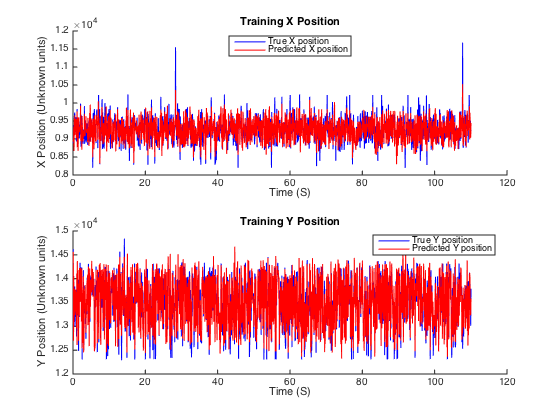
\includegraphics [width=4in]{mlautman_hw7_06.png}


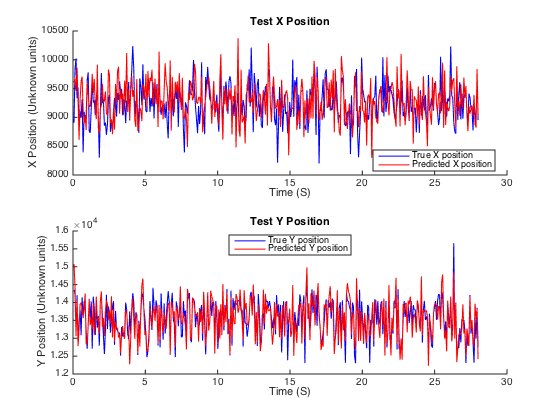
\includegraphics [width=4in]{mlautman_hw7_07.png}
\begin{par}

\subsection*{2.2.a Lasso}

\end{par}
\begin{lstlisting}
% predicting X positions
[f_lasso1, fit1]  = lasso(R_trn, s_trn(:,1), 'Lambda', 0.015);
non_zeros = sum(f_lasso1>0,1);
u_lasso1 = R_tst * f_lasso1;
rho_x_lasso = corr(s_tst(:,1),u_lasso1);

figure(9)
plot(non_zeros, rho_x_lasso);
title('Non Zero Feature Weights vs. Test Correlation')
xlabel('Non Zero Feature Weights')
ylabel('Test Correlation')
\end{lstlisting}


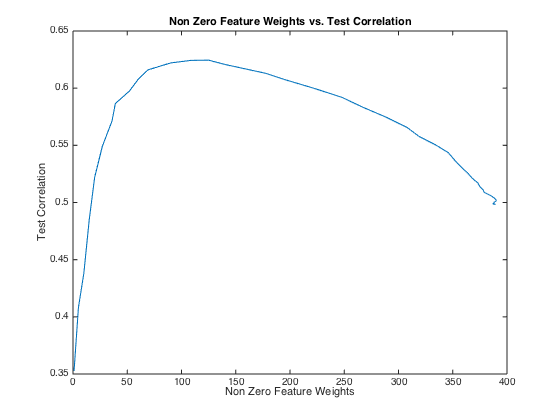
\includegraphics [width=4in]{mlautman_hw7_08.png}
\begin{par}

\subsection*{2.2.b How it works}
The additional L1 penalty for complexity in the model forces the
optimization to choose a set of coefficients that represent the ideal
function as closely as possible using as few coefficients as possible. By
increasing $\lambda$, we can increase the penalty for model
complexity and reduce the number of non-zero coefficients. By reducing
$\lambda$ we can have the opposite effect.

\end{par}
\begin{par}

\section*{3 Grand Challenge}
I tried two methods for predicting monkey hand positions. The first
method was linear regression with the lasso complexity penalty. This
method was able to be tuned to yeild correlation scores up to
aproximately 0.90 on the test set. The problem with this method is that a
linear combination of the input variables is most likely not the ideal
representation of the underlying system. In reality, the true function
space is much more complex than a linear combination can allow for. For
that reason, I applied a Nu-SVC regression with a radial basis function
kernel. Since the Matlab builtin SVC implementation does not support
regression I used an open source implementation initially written by Jun-
Cheng Chen, Kuan-Jen Peng, Chih-Yuan Yang and Chih-Huai Cheng from
Department of Computer Science, National Taiwan University. Using this
method I was able to tune my implementation to achieve correlation scores
upwards of 0.98 during cross validation.

\end{par}


\subsection*{Linear regression}

\begin{lstlisting}
load('HW7Data');
n_neur = size(test_count, 2);
N = 5; % backwards looking time stamps for each neuron for feature vect
d = n_neur * N + 1; % 40 neurons by 20 time steps plus a ones vect for bias
Mtrn = size(count,1) - N + 1;
R_trn = zeros(Mtrn, d);

Mtst = size(test_count,1) - N + 1; % last timestamp for positions
R_tst = zeros(Mtst, d);

scale = 1; % Scaling discretization bins
rand_test_set = false;
% We create the R trn matrix

for i=1:Mtrn
    e = i + N - 1;
    row = count(i:e, :);
    R_trn(i, :) = [1, row(:)'];
end

% We create the R tst matrix
for i=1:Mtst
    e = i + N - 1;
    row = test_count(i:e, :);
    R_tst(i, :) = [1, row(:)'];
end

% Randomize test set (or not)
if rand_test_set
    perm = randperm(size(R,1));
else
    perm = 1:size(R_trn,1);
end

% training set
R_trn = R_trn(perm, :);

% Training data NOT discretized
s_trn = angles(perm, :);

% Linear regression explicit solution
f_trn = pinv(R_trn' * R_trn) * (R_trn' * s_trn);

% predictions
u_tst = R_tst * f_trn;
u_trn = R_trn * f_trn;

% Solving for the correlation scores
rho2_x = corr(s_trn(:,1),u_trn(:,1));
rho2_y = corr(s_trn(:,2),u_trn(:,2));
rho2_z = corr(s_trn(:,3),u_trn(:,3));
c = corr(s_trn, u_trn);
\end{lstlisting}

\subsection*{Find best lambda x using CV}
\begin{lstlisting}
[Bx2_n,FitInfo1] = lasso(R_trn(:,2:size(R_trn,2)),s_trn(:,1),'NumLambda',5, 'CV', 5); 
lassoPlot(Bx2_n,FitInfo1,'PlotType','CV');

%% Build model for X 
[Bx,FitInfo_x] = lasso(R_trn(:,2:size(R_trn,2)), s_trn(:,1),'Lambda', 0.015); 
Bo = FitInfo_x.Intercept; 
Bx = [Bo;Bx]; 
predX_trn = R_trn * Bx; 
predX = R_tst * Bx; 
% rho_x = corr(s_tst(:,1), predX)

%% Find best lambda y through CV 
[By2_n,FitInfo1] = lasso(R_trn(:,2:size(R_trn,2)),s_trn(:,2),'NumLambda', 10, 'CV', 10); 
lassoPlot(By2_n,FitInfo1,'PlotType','CV');

%% Build model for Y 
[By,FitInfo_y] = lasso(R_trn(:, 2:size(R_trn,2)), s_trn(:,2),'Lambda', 0.015); 
Bo = FitInfo_y.Intercept; 
By = [Bo; By]; 
predY_trn = R_trn * By; 
predY = R_tst * By;
% rho_y = corr(s_tst(:,2), predY)

%% Find best lambda z through CV 
[By2_n,FitInfo1] = lasso(R_trn(:,2:size(R_trn,2)),s_trn(:,2),'NumLambda',10, 'CV', 10); 
lassoPlot(By2_n,FitInfo1,'PlotType','CV');

%% Build model for Z 
[Bz,FitInfo_z] = lasso(R_trn(:,2:size(R_trn,2)), s_trn(:,3),'Lambda',0.015); 
Bo = FitInfo_z.Intercept; Bz = [Bo ;Bz]; 
predZ_trn = R_trn * Bz; 
predZ = R_tst * Bz; 
% rho_z = corr(s_tst(:,3), predZ)
\end{lstlisting}

\begin{lstlisting}
%% Animate results
 
figure(10)
subplot(1,3,1);
hold on
axis([...
	min(s_trn(:,1)) max(s_trn(:,1)) ...
	min(s_trn(:,2)) max(s_trn(:,2)) ...
	min(s_trn(:,3)) max(s_trn(:,3)) ...
])
subplot(1,3,2);
hold on
axis([...
	min(predX_trn) max(predX_trn) ...
	min(predY_trn) max(predY_trn) ...
	min(predZ_trn) max(predZ_trn) ...
])
subplot(1,3,3);
hold on
axis([...
	min(predX) max(predX) ...
	min(predY) max(predY) ...
	min(predZ) max(predZ) ...
])
for i=1:min(length(predX), length(predX_trn))
    subplot(1,3,1);
	scatter3(s_trn(i,1), s_trn(i,2), s_trn(i,3))
	
    subplot(1,3,2);
    scatter3(predX_trn(i), predY_trn(i), predZ_trn(i))
    
    subplot(1,3,3);
	scatter3(predX(i), predY(i), predZ(i))
	pause(.01)
end
\end{lstlisting}


\subsection*{SVC}

\begin{lstlisting}
load('HW7Data');
n_neur = size(test_count, 2);
N = 20; % backwards looking time stamps for each neuron for feature vect
d = n_neur * N + 1; % 40 neurons by 20 time steps plus a ones vect for bias
Mtrn = size(count,1) - N + 1;
R_trn = zeros(Mtrn, d);

Mtst = size(test_count,1) ; % last timestamp for positions
R_tst = zeros(Mtst, d);

scale = 1; % Scaling discretization bins
rand_test_set = false;
% We create the R trn matrix


for i=1:Mtrn
    e = i + N - 1;
    row = count(i:e, :);
    R_trn(i, :) = [1, row(:)'];
end


% We create the R tst matrix
for i=1:Mtst
    e = i + N - 1;
    if e > Mtst
        e = Mtst;
    end
    row = test_count(i:e, :);
    r_h = size(row, 1);
    if r_h < N
        delta = N - r_h;
        for j = 1:delta
            row = [row; row(r_h,:)];
        end
    end
    R_tst(i, :) = [1, row(:)'];
end

% Randomize test set (or not)
if rand_test_set
    perm = randperm(size(R,1));
else
    perm = 1:size(R_trn,1);
end

% training set
R_trn = R_trn(perm, :);

% Training data NOT discretized
s_trn = angles(perm, :);
garbage_pred = ones(size(R_tst,1),1);
\end{lstlisting}


\subsection*{Useful functions for tuning parameters}

\begin{lstlisting}
svmX = svmtrain(round(s_trn(:,1)),R_trn, '-s 4 -t 2 -d 10 -c 100.5 -v 10 -q');
svmY = svmtrain(round(s_trn(:,2)),R_trn, '-s 4 -t 2 -d 10 -c 100.5 -v 10 -q');
svmZ = svmtrain(round(s_trn(:,3)),R_trn, '-s 4 -t 2 -d 10 -c 100.5 -v 10 -q');
\end{lstlisting}

\color{lightgray} \begin{lstlisting}Cross Validation Mean squared error = 0.347638
Cross Validation Squared correlation coefficient = 0.975629
Cross Validation Mean squared error = 1.24202
Cross Validation Squared correlation coefficient = 0.989913
Cross Validation Mean squared error = 0.76548
Cross Validation Squared correlation coefficient = 0.987479
\end{lstlisting} \color{black}


\subsection*{Train SVR X}

\begin{lstlisting}
svmX = svmtrain(round(s_trn(:,1)),R_trn, '-s 4 -t 2 -c 100.5 -q');
% make predictions on resulting set
predX_trn = svmpredict(s_trn(:,1), R_trn, svmX, '-q');
predX = svmpredict(garbage_pred, R_tst, svmX, '-q');
% svr_corr_X = corr(predX, s_tst(:,1))
% Train SVR Y
svmY = svmtrain(round(s_trn(:,2)),R_trn, '-s 4 -t 2 -c 100.5 -q');
% make predictions on resulting set
predY_trn = svmpredict(s_trn(:,2), R_trn, svmY, '-q');
predY = svmpredict(garbage_pred, R_tst, svmY, '-q');
% svr_corr_Y = corr(predY, s_tst(:,2))
% Train SVR Z
svmZ = svmtrain(round(s_trn(:,3)),R_trn, '-s 4 -t 2 -c 100.5 -q');
% make predictions on resulting set
predZ_trn = svmpredict(s_trn(:,3), R_trn, svmZ, '-q');
predZ = svmpredict(garbage_pred, R_tst, svmZ, '-q');
% svr_corr_Z = corr(predZ, s_tst(:,3))


%% Animate results
subplot(1,3,1);
hold on
axis([...
	min(s_trn(:,1)) max(s_trn(:,1)) ...
	min(s_trn(:,2)) max(s_trn(:,2)) ...
	min(s_trn(:,3)) max(s_trn(:,3)) ...
])
subplot(1,3,2);
hold on
axis([...
	min(predX_trn) max(predX_trn) ...
	min(predY_trn) max(predY_trn) ...
	min(predZ_trn) max(predZ_trn) ...
])
subplot(1,3,3);
hold on
axis([...
	min(predX) max(predX) ...
	min(predY) max(predY) ...
	min(predZ) max(predZ) ...
])
for i=1:min(length(predX), length(predX_trn))
	subplot(1,3,1);
	scatter3(s_trn(i,1), s_trn(i,2), s_trn(i,3))

	subplot(1,3,2);
	scatter3(predX_trn(i), predY_trn(i), predZ_trn(i))

	subplot(1,3,3);
	scatter3(predX(i), predY(i), predZ(i))
	pause(.01)
end

clf; clear all; close all;
\end{lstlisting}



\end{document}
    
